\documentclass[aspectratio=169,10pt]{beamer}
\usetheme{Madrid}
\usecolortheme{seahorse}

\usepackage[utf8]{inputenc}
\usepackage{amsmath,amssymb,amsthm}
\usepackage{listings}
\usepackage{xcolor}
\usepackage{graphicx}
\usepackage{hyperref}

\graphicspath{{figures/}}

\setbeamertemplate{navigation symbols}{}
\setbeamertemplate{footline}[frame number]

\lstset{
    language=Python,
    basicstyle=\ttfamily\scriptsize,
    keywordstyle=\color{blue},
    commentstyle=\color{green!50!black},
    stringstyle=\color{red},
    showstringspaces=false,
    numbers=left,
    numberstyle=\tiny\color{gray},
    frame=single,
    breaklines=true,
    tabsize=2
}

\title{Discrete and Topological Structures}
\subtitle{Chapter 1a: Pathak's Introduction to Nonlinear Analysis}
\author{Based on H.K. Pathak (2018)}
\date{2026}

\begin{document}

\frame{\titlepage}

\begin{frame}
\frametitle{Outline}
\tableofcontents[hideallsubsections]
\end{frame}

\section{Section 1.1: Discrete Structure}

\begin{frame}
\frametitle{Partially Ordered Sets}

\begin{definition}[Partial Order]
A binary relation $\preceq$ on a nonempty set $X$ is a \emph{partial order} if:
\begin{itemize}
\item[\textbf{P1}] Reflexive: $x \preceq x$ for all $x \in X$
\item[\textbf{P2}] Antisymmetric: $x \preceq y$ and $y \preceq x$ imply $x = y$
\item[\textbf{P3}] Transitive: $x \preceq y$ and $y \preceq z$ imply $x \preceq z$
\end{itemize}
\end{definition}

A \emph{partially ordered set} or \emph{poset} is a set with a partial order, denoted $(X, \preceq)$.

\vspace{0.3cm}

\textbf{Examples:}
\begin{itemize}
\item Standard order $\leq$ on $\mathbb{R}$
\item Subset relation $\subseteq$ on power sets
\item Divisibility on positive integers
\end{itemize}
\end{frame}

\begin{frame}
\frametitle{Chains and Extremal Elements}

\begin{definition}
\begin{itemize}
\item A \emph{chain} is a totally ordered subset
\item An \emph{upper bound} of $S$ is an element $u$ such that $s \preceq u$ for all $s \in S$
\item A \emph{least upper bound} (supremum) is the smallest upper bound
\item An element is \emph{maximal} if no larger element exists
\item An element is \emph{minimal} if no smaller element exists
\end{itemize}
\end{definition}

\vspace{0.3cm}

\begin{columns}[T]
\column{0.5\textwidth}
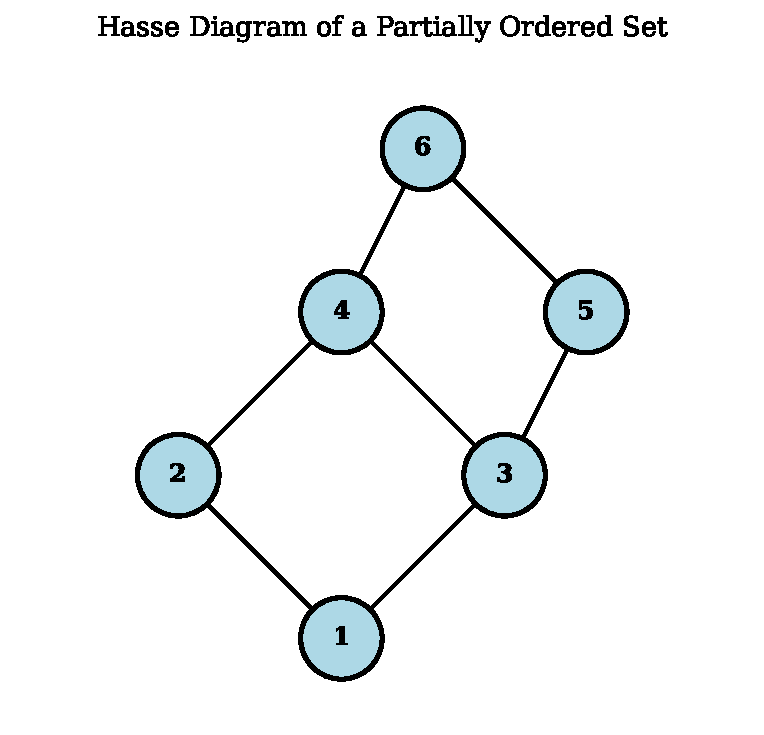
\includegraphics[width=\textwidth]{fig_poset.pdf}

\column{0.5\textwidth}
\textbf{Key Properties:}
\begin{itemize}
\item Maximal elements may not be unique
\item A maximum element (if it exists) is maximal
\item In a total order, maximal = maximum
\end{itemize}
\end{columns}
\end{frame}

\begin{frame}
\frametitle{Zorn's Lemma}

\begin{theorem}[Zorn's Lemma]
If $(X, \preceq)$ is a poset where every chain has an upper bound, then $X$ has a maximal element.
\end{theorem}

\vspace{0.3cm}

\textbf{Significance:}
\begin{itemize}
\item Equivalent to the Axiom of Choice
\item Essential for existence proofs in functional analysis
\item Used in Hahn-Banach theorem, basis existence, maximal ideals
\end{itemize}
\end{frame}

\begin{frame}
\frametitle{Lattices}

\begin{definition}[Lattice]
A \emph{lattice} is a poset $(A, \preceq)$ where for any $a, b \in A$:
\begin{itemize}
\item Their \emph{join} (least upper bound) $a \vee b$ exists
\item Their \emph{meet} (greatest lower bound) $a \wedge b$ exists
\end{itemize}
\end{definition}

A lattice is \emph{complete} if every subset has a supremum and infimum.

\vspace{0.3cm}

\begin{columns}[T]
\column{0.5\textwidth}
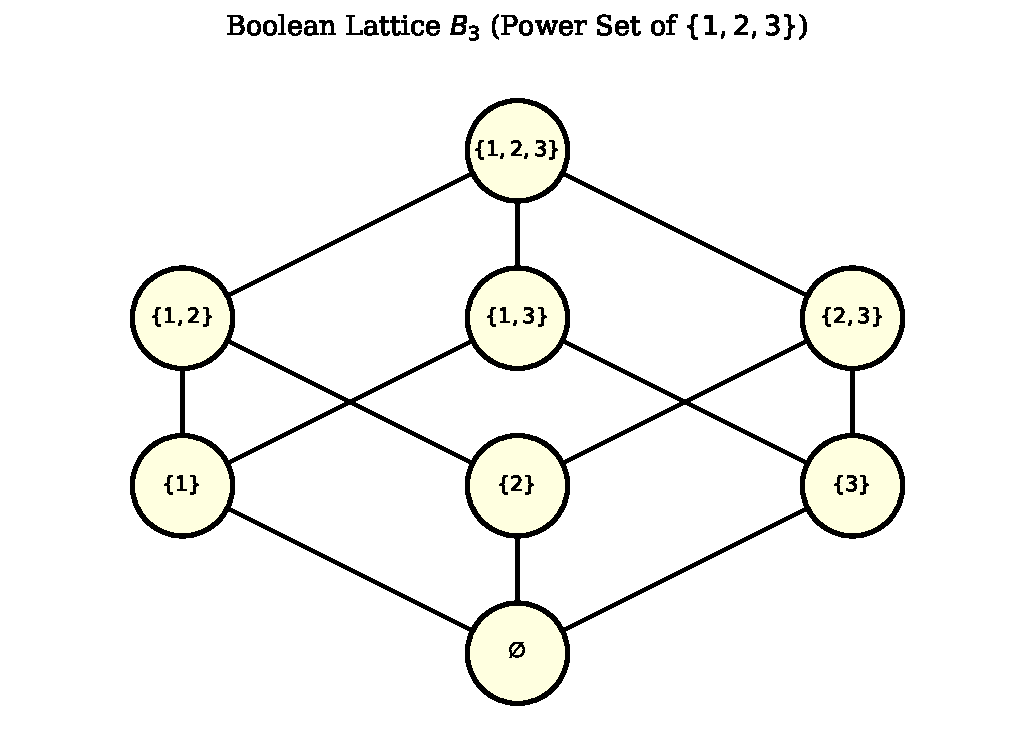
\includegraphics[width=\textwidth]{fig_lattice.pdf}

\column{0.5\textwidth}
\textbf{Example: Power Set}
\begin{itemize}
\item Elements: All subsets of $\{1,2,3\}$
\item Join: Union
\item Meet: Intersection
\item Minimum: $\emptyset$
\item Maximum: $\{1,2,3\}$
\end{itemize}
\end{columns}
\end{frame}

\section{Section 1.2: Topological Spaces}

\begin{frame}
\frametitle{Metric Spaces}

\begin{definition}[Metric]
A function $d: X \times X \to \mathbb{R}$ is a \emph{metric} if for all $x, y, z \in X$:
\begin{itemize}
\item[\textbf{M1}] $d(x,y) \geq 0$ (non-negativity)
\item[\textbf{M2}] $d(x,y) = 0 \iff x = y$ (identity)
\item[\textbf{M3}] $d(x,y) = d(y,x)$ (symmetry)
\item[\textbf{M4}] $d(x,y) \leq d(x,z) + d(z,y)$ (triangle inequality)
\end{itemize}
\end{definition}

A \emph{metric space} is a pair $(X, d)$ where $d$ is a metric.

\vspace{0.3cm}

\textbf{Examples:}
\begin{itemize}
\item Euclidean distance: $d(x,y) = |x-y|$ on $\mathbb{R}$
\item Discrete metric: $d(x,y) = \begin{cases} 0 & x=y \\ 1 & x \neq y \end{cases}$
\end{itemize}
\end{frame}

\begin{frame}
\frametitle{Open Sets and Continuity}

\begin{definition}[Open Ball and Open Set]
An \emph{open ball} around $x$ with radius $r$ is:
$$B(x, r) = \{y \in X : d(x,y) < r\}$$

A set $G$ is \emph{open} if for every $x \in G$, there exists $r > 0$ with $B(x,r) \subseteq G$.
\end{definition}

\vspace{0.3cm}

\begin{definition}[Continuity]
$f: X \to Y$ is \emph{continuous at} $x_0$ if for every $\epsilon > 0$, there exists $\delta > 0$ such that:
$$d_X(x, x_0) < \delta \implies d_Y(f(x), f(x_0)) < \epsilon$$
\end{definition}

\vspace{0.3cm}

\begin{columns}[T]
\column{0.5\textwidth}
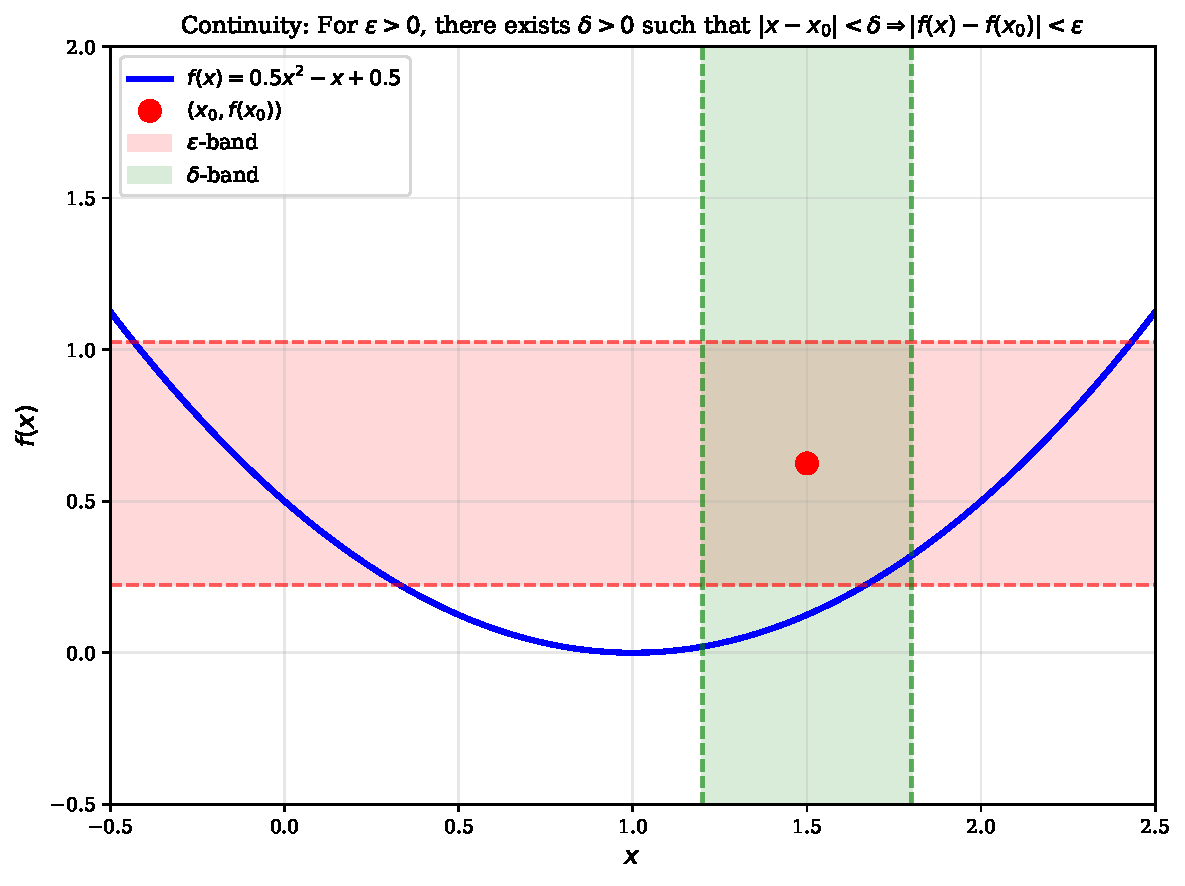
\includegraphics[width=\textwidth]{fig_continuity.pdf}

\column{0.5\textwidth}
\textbf{Equivalent characterization:}

$f$ is continuous iff the preimage of every open set is open.
\end{columns}
\end{frame}

\begin{frame}
\frametitle{Semicontinuity}

\begin{definition}[Semicontinuous Functions]
A function $\varphi: X \to \mathbb{R}$ is:
\begin{itemize}
\item \emph{Upper semicontinuous} at $x_0$ if $\limsup_{x \to x_0} \varphi(x) \leq \varphi(x_0)$
\item \emph{Lower semicontinuous} at $x_0$ if $\liminf_{x \to x_0} \varphi(x) \geq \varphi(x_0)$
\item \emph{Continuous} if both conditions hold
\end{itemize}
\end{definition}

\vspace{0.3cm}

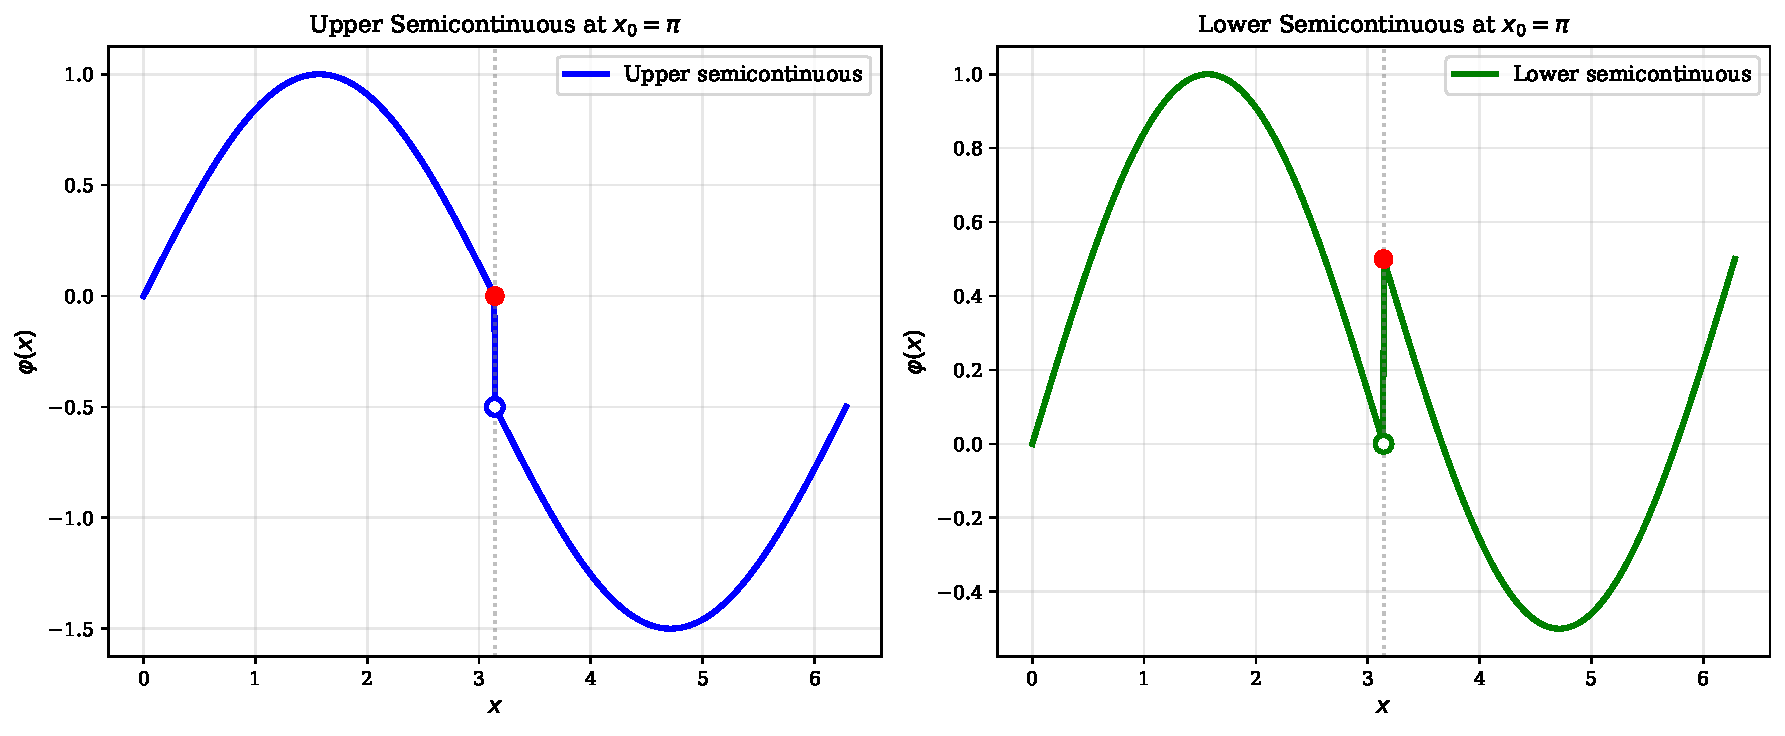
\includegraphics[width=\textwidth]{fig_semicontinuity.pdf}
\end{frame}

\begin{frame}
\frametitle{Closed Sets and Closure}

\begin{definition}[Closed Set]
A set $F$ is \emph{closed} if its complement $X \setminus F$ is open.
\end{definition}

\begin{definition}[Closure]
The \emph{closure} $\overline{C}$ of a set $C$ is the intersection of all closed sets containing $C$.
\end{definition}

\vspace{0.3cm}

\textbf{Properties:}
\begin{itemize}
\item A set is closed iff $C = \overline{C}$
\item The closed ball $\overline{B}(x,r) = \{y : d(x,y) \leq r\}$ is closed
\item Closure is the ``smallest'' closed set containing $C$
\item Intersection of closed sets is closed
\end{itemize}
\end{frame}

\begin{frame}
\frametitle{Neighborhoods and Separation Axioms}

\begin{definition}[Neighborhood]
$N$ is a \emph{neighborhood} of $x$ if there exists an open set $G$ with $x \in G \subseteq N$.
\end{definition}

\vspace{0.3cm}


\includegraphics[width=\textwidth]{fig_separation.pdf}

Separation axioms allow distinguishing points using open sets.
\end{frame}

\begin{frame}
\frametitle{Nets and Convergence}

\begin{definition}[Directed Set]
$(\mathcal{D}, \geq)$ is directed if it's reflexive, transitive, and for any $\alpha, \beta \in \mathcal{D}$, there exists $\gamma$ with $\gamma \geq \alpha, \beta$.
\end{definition}

\begin{definition}[Net]
A \emph{net} is a function from a directed set into $X$. The net $\{x_\alpha\}$ converges to $x$ if for every neighborhood $U$ of $x$, there exists $\alpha_0$ such that $x_\alpha \in U$ for all $\alpha \geq \alpha_0$.
\end{definition}

\vspace{0.3cm}

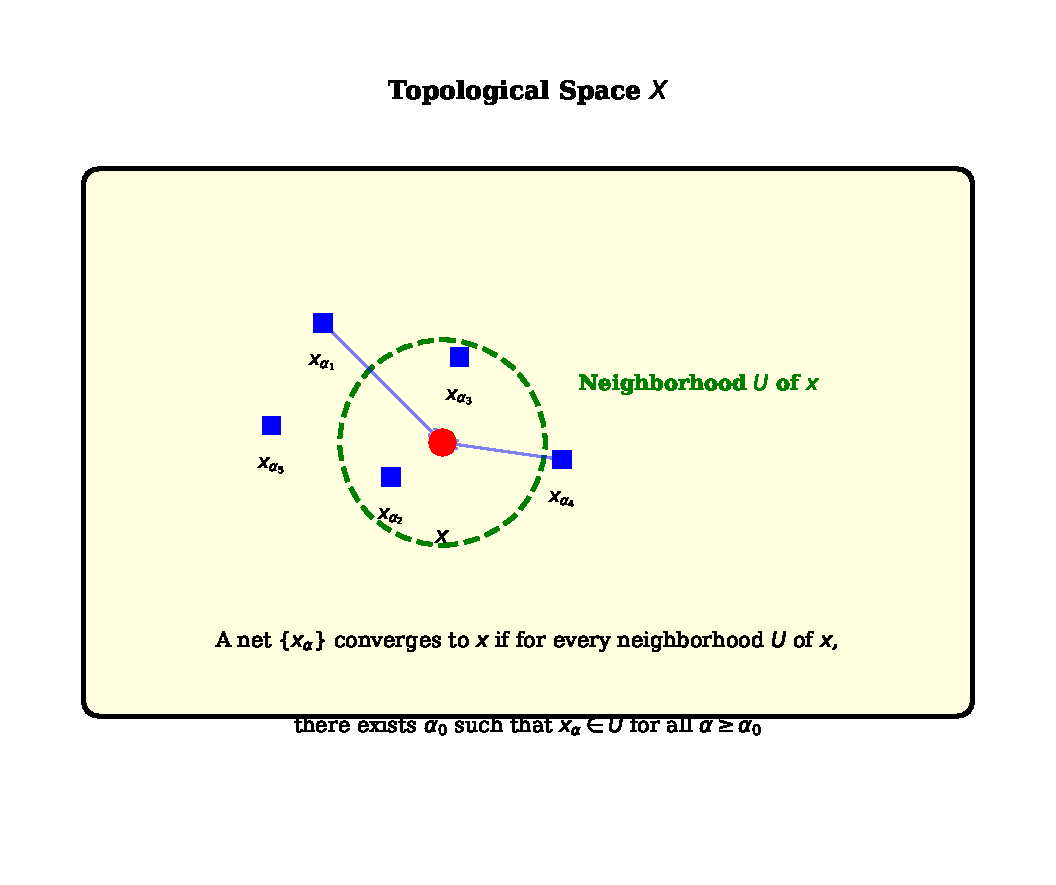
\includegraphics[width=\textwidth]{fig_net.pdf}
\end{frame}

\begin{frame}
\frametitle{Compactness}

\begin{definition}[Compact Space]
A space $X$ is \emph{compact} if every open cover has a finite subcover.
\end{definition}

\vspace{0.3cm}

\begin{theorem}[Heine-Borel]
A subset of $\mathbb{R}^n$ is compact iff it is closed and bounded.
\end{theorem}

\vspace{0.3cm}

\textbf{Key properties:}
\begin{itemize}
\item Continuous image of compact space is compact
\item In compact Hausdorff spaces, limits are unique
\item $[a,b]$ is compact in $\mathbb{R}$; $(a,b)$ is not
\end{itemize}

\vspace{0.3cm}

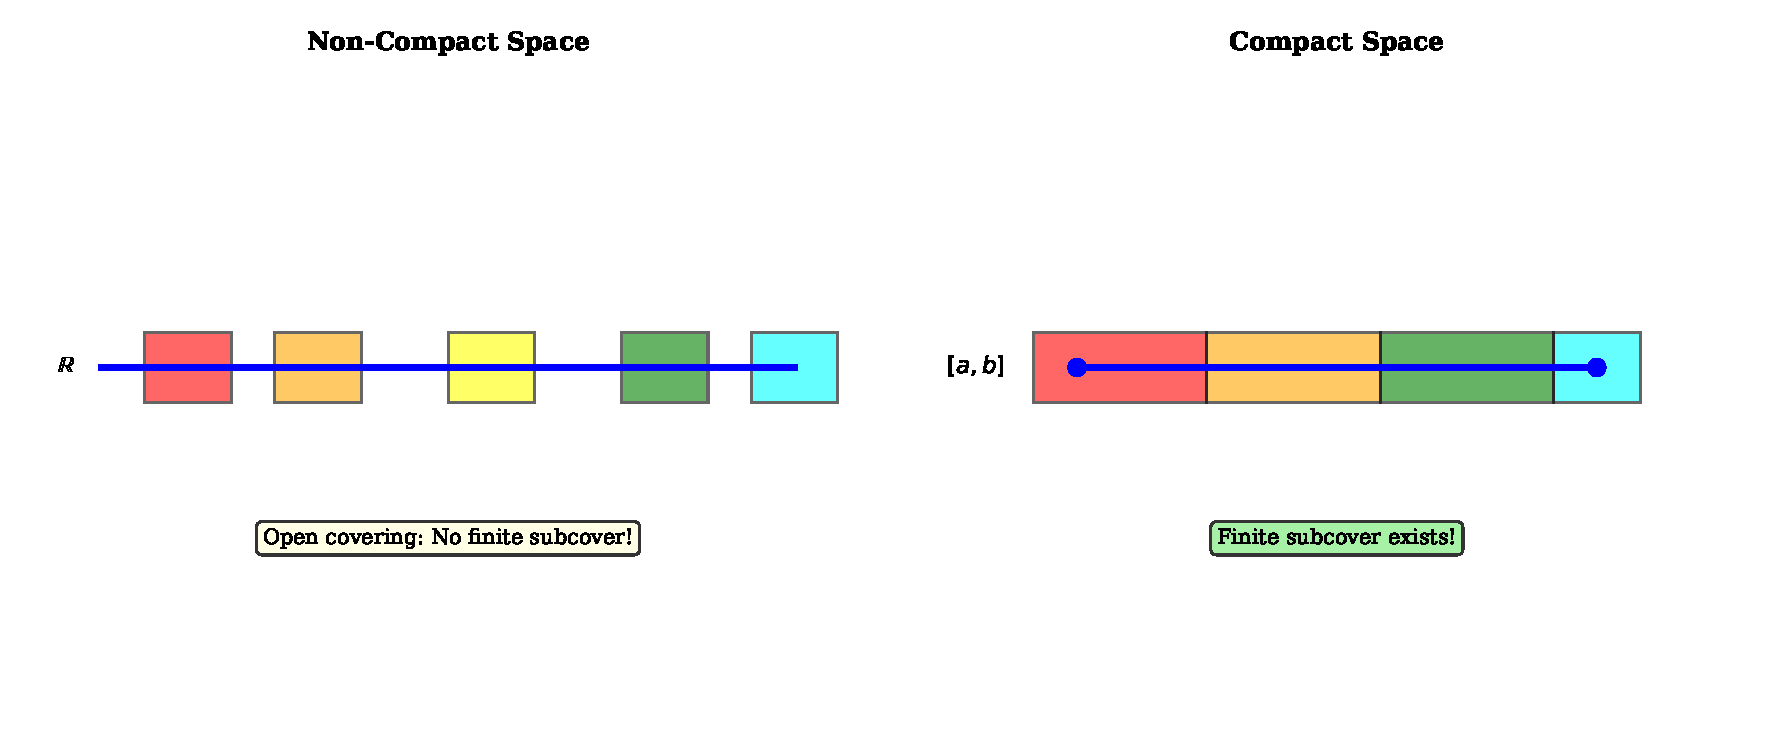
\includegraphics[width=\textwidth]{fig_compactness.pdf}
\end{frame}

\begin{frame}
\frametitle{Normed Linear Spaces}

\begin{definition}[Norm]
A function $\|\cdot\|: X \to [0, \infty)$ on a linear space is a \emph{norm} if:
\begin{itemize}
\item[\textbf{N1}] $\|x\| = 0 \iff x = 0$
\item[\textbf{N2}] $\|\lambda x\| = |\lambda| \|x\|$
\item[\textbf{N3}] $\|x + y\| \leq \|x\| + \|y\|$
\end{itemize}
\end{definition}

Every normed space is a metric space with $d(x,y) = \|x - y\|$.

\vspace{0.3cm}

\textbf{Common norms on} $\mathbb{R}^n$:
\begin{itemize}
\item $\|x\|_1 = \sum_i |x_i|$ (Manhattan norm)
\item $\|x\|_2 = \sqrt{\sum_i |x_i|^2}$ (Euclidean norm)
\item $\|x\|_\infty = \max_i |x_i|$ (Chebyshev norm)
\end{itemize}
\end{frame}

\begin{frame}
\frametitle{Unit Spheres in Different Norms}

The \emph{unit sphere} is $S = \{x : \|x\| = 1\}$. Its shape depends on the norm:

\vspace{0.3cm}

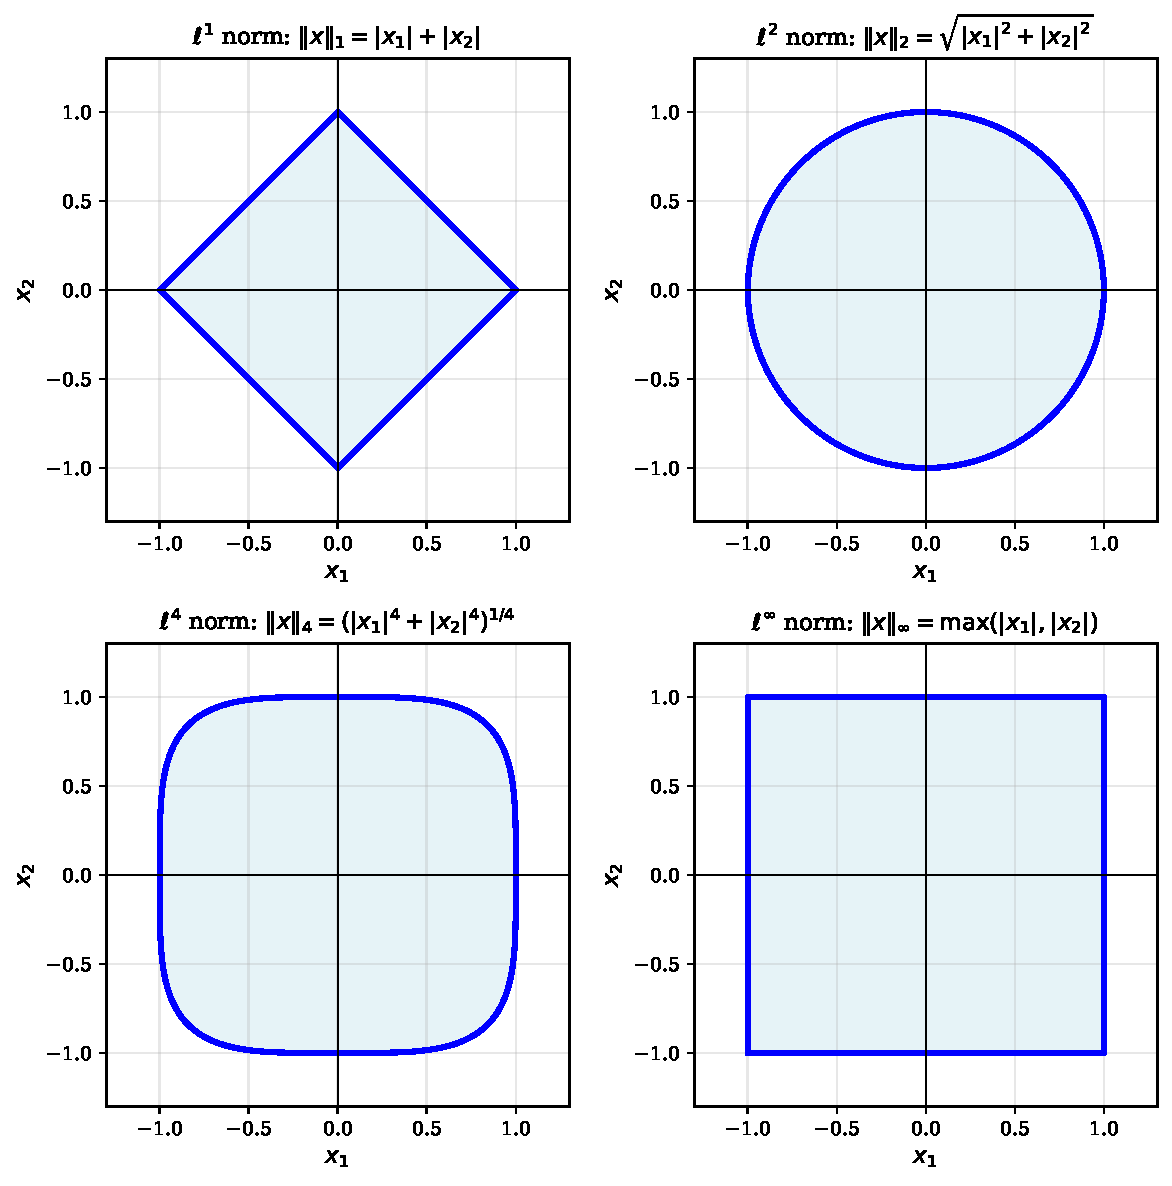
\includegraphics[width=\textwidth]{fig_unit_spheres.pdf}

All $\ell^p$ norms on $\mathbb{R}^n$ are \emph{equivalent} (generate the same topology).
\end{frame}

\begin{frame}
\frametitle{Inner Product Spaces}

\begin{definition}[Inner Product]
A function $\langle \cdot, \cdot \rangle: X \times X \to \mathbb{C}$ is an \emph{inner product} if:
\begin{itemize}
\item[\textbf{IP1}] $\langle x, x \rangle \geq 0$ for all $x$
\item[\textbf{IP2}] $\langle x, x \rangle = 0 \iff x = 0$
\item[\textbf{IP3}] $\langle x, y \rangle = \overline{\langle y, x \rangle}$
\item[\textbf{IP4}] Linear in first argument
\end{itemize}
\end{definition}

Every inner product induces a norm: $\|x\| = \sqrt{\langle x, x \rangle}$.

\vspace{0.3cm}

\textbf{Example:} On $\mathbb{R}^n$,
$$\langle x, y \rangle = \sum_{i=1}^n x_i y_i$$
\end{frame}

\begin{frame}[fragile]
\frametitle{Example: The Hilbert Space $\ell^2$}

\begin{definition}[$\ell^2$ Space]
$$\ell^2 = \left\{(x_i)_{i=1}^\infty : \sum_{i=1}^\infty |x_i|^2 < \infty\right\}$$
\end{definition}

With inner product: $\langle x, y \rangle = \sum_{i=1}^\infty x_i \overline{y_i}$.

\vspace{0.3cm}

\begin{lstlisting}[language=Python]
import numpy as np

# Example: x = (1, 1/2, 1/4, 1/8, ...)
x = np.array([1/2**i for i in range(1, 20)])

# Compute l^2 norm
norm_x = np.linalg.norm(x)
sum_sq = np.sum(x**2)

print(f"||x||_2 = {norm_x:.6f}")
print(f"Sum x_i^2 = {sum_sq:.6f}")

# Geometric series sums to 1/3
theoretical = 1/(1 - 1/4)
print(f"Limit = {theoretical:.6f}")
\end{lstlisting}
\end{frame}

\section{Summary}

\begin{frame}
\frametitle{Key Concepts}

\textbf{Discrete Structures (1.1):}
\begin{itemize}
\item Partially ordered sets and chains
\item Zorn's lemma for maximal elements
\item Lattices with joins and meets
\end{itemize}

\vspace{0.3cm}

\textbf{Topological Foundations (1.2):}
\begin{itemize}
\item Metric spaces and distances
\item Open/closed sets and continuity
\item Compactness and completeness
\item Normed and inner product spaces
\end{itemize}

\vspace{0.3cm}

These tools are fundamental for:
\begin{itemize}
\item Nonlinear functional analysis
\item Fixed point theorems
\item Optimization and variational methods
\end{itemize}
\end{frame}

\begin{frame}
\frametitle{References}

\begin{thebibliography}{99}
\bibitem{pathak2018}
Pathak, H.K. (2018). \textit{An Introduction to Nonlinear Analysis and Fixed Point Theory}. Springer.

\bibitem{rudin1976}
Rudin, W. (1976). \textit{Principles of Mathematical Analysis}. McGraw-Hill.

\bibitem{munkres2000}
Munkres, J.R. (2000). \textit{Topology}. Prentice Hall.
\end{thebibliography}
\end{frame}

\end{document}
